\documentclass[12pt,a4paper]{article}

\usepackage[dvipsnames]{xcolor}
\usepackage[utf8]{inputenc}
\usepackage[T1]{fontenc}
\usepackage[top=3cm, bottom=4.5cm, left=2.8cm, right=2.8cm]{geometry}
\usepackage[pdftex]{graphicx}
\usepackage[english]{babel}
\usepackage{amssymb, amsmath, mathtools}
\usepackage{subcaption}
\usepackage{color}
\usepackage{siunitx}
\usepackage{fancyhdr}
\usepackage{svg}
\usepackage{hyperref}
\usepackage[english]{cleveref}
\usepackage{hhline}
\usepackage{colortbl}
\usepackage{wrapfig}
\usepackage{listings}
\usepackage[style=alphabetic]{biblatex}
\usepackage{csquotes}

\addbibresource{bibliography.bib}
\graphicspath{{images/}}
\renewcommand{\labelenumii}{\arabic{enumi}.\arabic{enumii}}

\pagestyle{fancyplain}
\headheight 35pt
\lhead{Politecnico di Torino}
%\chead{\today}
\rhead{GPU Programming}
\lfoot{}
\cfoot{}

\setlength{\intextsep}{6pt}

\renewcommand{\arraystretch}{1.3}

% Modulo ----------------------------------------
\DeclarePairedDelimiter\abs{\lvert}{\rvert}%
\DeclarePairedDelimiter\norm{\lVert}{\rVert}%

% Swap the definition of \abs* and \norm*, so that \abs
% and \norm resizes the size of the brackets, and the 
% starred version does not.
\makeatletter
\let\oldabs\abs
\def\abs{\@ifstar{\oldabs}{\oldabs*}}
%
\let\oldnorm\norm
\def\norm{\@ifstar{\oldnorm}{\oldnorm*}}
\makeatother
% -----------------------------------------------

\begin{document}

\begin{figure}[b]
\centering

\includegraphics[width=0.35\textwidth]{logo_polito}
\end{figure}

%\begin{vplace}[0.15]
\title{Unbiased, progressive path tracing in CUDA with Next Event Estimation and BVH accelerated ray tracing}
\author{}
\maketitle
\vspace{10cm}
\begin{center}Davide Miola\\Cristiano Canepari\end{center}
%\end{vplace}

\newpage

\tableofcontents
\newpage

\setcounter{page}{1}
\rfoot{\thepage}
%\thispagestyle{myheadings}

\section{Abstract}

We explore ray tracing in CUDA by building a progressive path tracer, i.e. an unbiased, Monte Carlo based approach to solve the rendering equation (\cite{10.1145/15886.15901}, \cite{10.1145/15886.15902}) by shooting millions of rays through a virtual camera, bouncing them across the scene's geometry according to the surfaces' material properties, and accumulating their contribution to progressively clean up the rendering artifact.

The CUDA program receives as input the description of the scene and virtual camera properties through an obj+mtl file combo, and produces as output a live view of the converging image (path tracing) by leveraging the CUDA capabilities of inter-operating with the Vulkan graphics API.

Special consideration is given to assessing the performance improvement yielded by employing a BVH (Bounding Volume Hierarchy) - an industry-standard, scalable acceleration structure used to speed up ray tracing - with respect to a brute force ray-geometry intersection algorithm.

\section{Related work}

Producing photo-realistic synthetic images of virtual 3D worlds is something that's been the focus of much research for many decades. Ultimately, this comes down to simulating the behavior of light rays bouncing around the geometry of the scene, and into a camera sensor. In 1986, the issue was formalized in the \textit{rendering equation} (\cite{10.1145/15886.15901}, \cite{10.1145/15886.15902}),
$$L_o(\vec{x}, \omega_o, \lambda, t)=L_e(\vec{x}, \omega_o, \lambda, t)+\int_{\Omega}f_r(\vec{x}, \omega_i, \omega_o, \lambda, t)L_i(\vec{x}, \omega_i, \lambda, t)(\omega_i \cdot \vec{n}) d\omega_i$$
which characterizes the radiance $L_o$ output from a surface point $\vec{x}$ in direction $\omega_o$ by an integral over the hemisphere defined by $\vec{x}$ and its surface normal $\vec{n}$.

A generalized analytical solution of the above integral doesn't exist, but many unbiased Monte Carlo based methods have been proposed throughout the years to solve the rendering equation numerically. Among these, Path Tracing (\cite{10.1145/15886.15902}) is arguably the most straightforward. In its most common form (\textit{backwards} path tracing), rays are shot from the camera pixels into the scene, and samples become meaningful only after randomly hitting a light source; on the other hand, the reverse is also possible (\textit{forwards} path tracing, or \textit{light tracing}), where rays originate from the lights, and scatter around until hitting the camera sensor.

Both of these methods are a special case of Bi-Directional Path Tracing (\cite{bidir}), in which a path is generated by tracing rays both from the camera and a light, and then merging the two at a midpoint. This provides lower variance, and is thus able to converge faster. Metropolis Light Transport (\cite{10.1145/258734.258775}) is another variation on top of Bi-Directional Path Tracing, where after a full path has been constructed, small variations are built from it; this proves very useful for exploiting difficult-to-find light paths and resolving otherwise problematic effects like caustics. Many modern commercial renderers use this technology.

\section{Proposed method}

Our work focuses on the development of a proof-of-concept backwards path tracer for Nvidia GPUs with CUDA. Delegating rendering to the video card has become quite common in the field, not only in the real time domain; this is because the massive parallelism of the GPU is well suited for this kind of task, as there are no dependencies between pixels, and thus they can be freely scheduled on different threads. Ray tracing is in fact an embarrassingly parallel algorithm, only limited by the resolution of the output image.

\subsection{Basic algorithm}
\label{sec:alg}

Our path tracer is \textit{progressive}, meaning that it never really stops on its own, but rather it keeps on accumulating samples until it's explicitly terminated. Because of this, the main kernel responsible for rendering the image (\verb|pathTrace() - app/path_tracing.cuh|) is continuously being called in a loop, with the CPU-GPU synchronization controlled by a CUDA \verb|Event|. Each launch of the kernel (a \textit{batch}) is responsible for accumulating a number of samples equal to the \verb|SAMPLES_PER_BATCH| constant (\verb|app/utils.cuh|, 32 by default), for each pixel of the framebuffer. Because every thread corresponds to only one pixel of the image, we went with a two dimensional grid to ease the allocation logic.

Following is a high level overview of the algorithm executed for every pixel:
\begin{enumerate}
\item Trace a new path with initial throughput of $1$ and black color:
    \begin{enumerate}
    \item Build the ray $r$ from the camera parameters and pixel id. This is the ray that originates in the camera's sensor and shoots out through the screen pixel.
    \item Match ray $r$ with all the triangles in the scene, looking for the closest intersection $\Vec{x}$. This step is called \textit{ray tracing}, and with this naive implementation it's not able to scale efficiently with the number of triangles. We provide a solution in the form of a \textit{BVH} (see section \ref{sec:bvh}).
    \item Integrate the path's color with the hit's emissive light $L_e$, multiplied by the path's throughput.
    \item Choose a random direction $\omega_i$ in $\Omega$, with a \textit{probability density function} $p$ (for a uniform distribution over the hemisphere $\Omega$, $p=\frac{1}{2\pi}$).
    \item Scale the path's throughput by the \textit{Bidirectional Reflectance Distribution Function} $f_r$ (\cite{wiki:Bidirectional_reflectance_distribution_function}) of the hit's material; this is the function that describes how light is reflected by an opaque surface. Note that for purely diffuse materials (as in our renderer), this is hugely simplified: the \textit{Lambertian brdf} is in fact just the constant $\frac{\rho}{\pi}$, where $\rho$, the material's \textit{albedo}, is the measure of its diffuse reflectance, i.e. its color.
    
    The throughput must also be scaled by the inverse of the pdf $p$ of $\omega_i$, to comply with the Monte Carlo method.
    \item Build the output ray $r$ with origin $\Vec{x}$ and direction $\omega_i$.
    \item Repeat from 1.2 until reaching the set bounce limit.

    Note that, instead of abruptly terminating paths - which would introduce a bias in the renderer - our implementation employs a so called \textit{Russian Roulette}, a technique which terminates paths by random chance, and boosts the throughput of surviving paths to regain the lost energy.
    \end{enumerate}
\item Average the path's final color into the pixel's framebuffer texel.
\item Repeat from 1. In the actual implementation, the first hit of every path is cached, to reduce the amount of ray tracing needed.
\end{enumerate}

\subsection{Cosine-weighted sampling}

One first small optimization comes in the form of a kind of \textit{Importance Sampling}, i.e. a family of techniques that aim to improve the way samples are allocated on the $\Omega$ hemisphere.

In this case, instead of the simple uniform distribution, we choose a cosine-weighted sampler, which will increase the chance of returning directions closer to $\Vec{n}$. This is beneficial because of the presence of the $(\omega_i \cdot \vec{n})$ term in the rendering equation, which implies that light hitting a surface at a shallow angle will weight \textit{less} than that coming perpendicularly; this is known as the \textit{Fresnel effect}. This way, we minimize the time spent tracing rays with a low throughput.

The probability density function $p$ of this distribution is $\frac{\omega_i \cdot \vec{n}}{\pi}$, which is particularly convenient, as it will all cancel out with the rendering equation's cosine term and Lambertian brdf's denominator.

\subsection{Next event estimation}

The main idea of next event estimation (also known as \textit{explicit light sampling}) - which is also a form of importance sampling - is to split the integration of direct and indirect lighting. For every path, at each of its bounces we randomly select a light-emitting triangle, and then sample that triangle directly, tracing a \textit{shadow ray}. It's important to then discard any eventual emission contribution from the "normal" flow underlined in section \ref{sec:alg}, because otherwise we would get double the amount of light.

The total number of rays traced per path roughly doubles, but we still expect next event estimation to provide much faster convergence rates, especially in scenes with smaller light sources, which would be hard to reach by pure chance otherwise. A notable detail in our implementation is that we allow the user to disable the feature, by defining \verb|NO_NEXT_EVENT_ESTIMATION| at compile time.

\subsection{Bounding Volume Hierarchy}
\label{sec:bvh}

A critical shortcoming that limits the real-world applicability of the naive algorithm depicted above is the ray-tracing implementation. Simply iterating through all the primitives in the scene to find the closest intersection for every ray is impractically inefficient, and only serviceable for small, simple scenes.

A very common solution is the employment of a so called \textit{acceleration structure} which, at its core, consists of a specialized and optimized representation of the scene's geometry in memory that allows faster and more efficient access for the ray tracing use-case. Many different kinds of acceleration structures have been proposed throughout the years, with more recent development focusing on space constraints and flexibility.

We decided to go for a tried and tested approach: the \textit{Bounding Volume Hierarchy}, or \textit{BVH} for short. This is an industry-standard acceleration structure that also happens to map really well to the GPU architecture, which is the reason why most - if not all - implementations of hardware accelerated ray tracing found in today's GPU hardware rely on BVHs for ray traversal. In practice, a BVH is a balanced binary tree that groups nearby primitives together under a common \textit{"bounding volume"}, which completely encloses the contained geometry. In most cases - like our implementation - the volume is an \textit{Axis Aligned Bounding Box} (or just \textit{AABB}), which greatly simplifies their management. A BVH traversal thus has a logarithmic time complexity with respect to the total number of primitives, while also substituting most ray-triangle intersection checks with faster and more efficient ray-AABB checks.

We opted to build the BVH on the CPU right after loading the scene from the file system and decoding the obj file format, and later upload the resulting structure to the GPU. Even though we were able to pack both internal and leaf nodes of the tree in as little as \qty{32}{\byte}, the BVH is still the biggest contributor to the GPU memory requirements by far.

An extra optimization enabled by the BVH on CUDA is the ability it unlocks to use shared memory, by loading the first few nodes of the structure in the faster memory pool. This is beneficial because the higher-level nodes are accessed more often than the deeper ones, as they are shared with more primitives. Our testing revealed that using as much shared memory as is available seems to provide the best results, even when the faster memory is shared with SM cache, and even if doing so would decrease the theoretical occupancy.

As for next event estimation, the BVH can disabled with \verb|NO_BVH|.

\subsection{Vulkan interface and PNG encoding}

A defining feature of our path tracer is its ability to show the real time progress via a Vulkan window. The way this is achieved is by sharing a GPU memory buffer allocated on the CUDA side with a Vulkan library, which then simply renders a traditional \textit{"full-screen quad"} to run a fragment shader that dumps the contents of this buffer to the current swapchain image (and, in doing so, leverages the GPU's ability to automatically perform gamma correction). As the Vulkan side accesses the shared buffer in a read-only fashion, no particular synchronization mechanism is required.

Two ways to share GPU memory between CUDA and Vulkan are available; the preferred one makes use of CUDA 10.2's virtual memory driver API feature, which allows to allocate exportable memory as O.S.-specific opaque handles. The alternative - introduced to ensure support for the Jetson Nano platform - instead uses "Zero-Copy" memory. The latter approach shares memory through the system RAM, by making a CPU buffer accessible from the GPU. This is acceptable on a unified memory platform like the Jetson, where Zero-Copy memory just disables caching, but would be catastrophically inefficient on traditional systems, and is better avoided.

Another output provided by the renderer is the ability to encode PNG images on exit. Note that this requires us to explicitly perform sRGB gamma correction to match the color profile offered "for free" by Vulkan.

\section{Results}

Results for a rendering solution have to be discussed separately for quality and speed. Being this an \textit{unbiased} path tracer, though, the quality of a converged image \textit{will} be equivalent to that of any other unbiased renderer, by definition. Our path tracer does not surprise here: in the example presented in \Cref{img:cornell_box_comparison}, a rendering of the iconic Cornell Box (\cite{site:Cornell_box}, \cite{wiki:Cornell_box}) is compared between our path tracer (\textit{left}), Blender Cycles 3.4.0 (\textit{middle}), and LuxCoreRender 2.61 (\textit{right}), showing an indistinguishable output.

\begin{figure}[h]
\centering
\begin{subfigure}{0.3\textwidth}
\centering
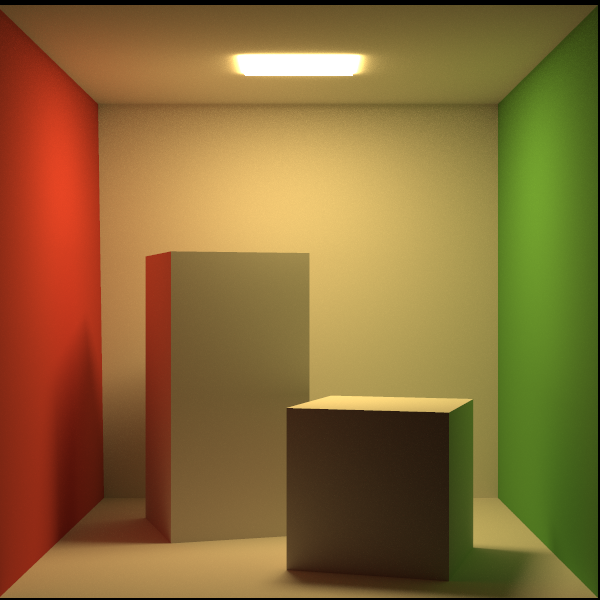
\includegraphics[width=\textwidth]{cornell_box_own.png}
\end{subfigure}
\hspace{0.2cm}
\begin{subfigure}{0.3\textwidth}
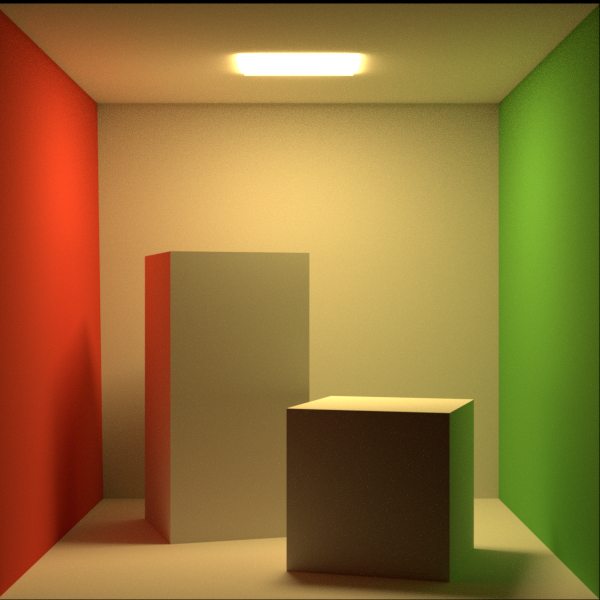
\includegraphics[width=\textwidth]{cornell_box_cycles.png}
\end{subfigure}
\hspace{0.2cm}
\begin{subfigure}{0.3\textwidth}
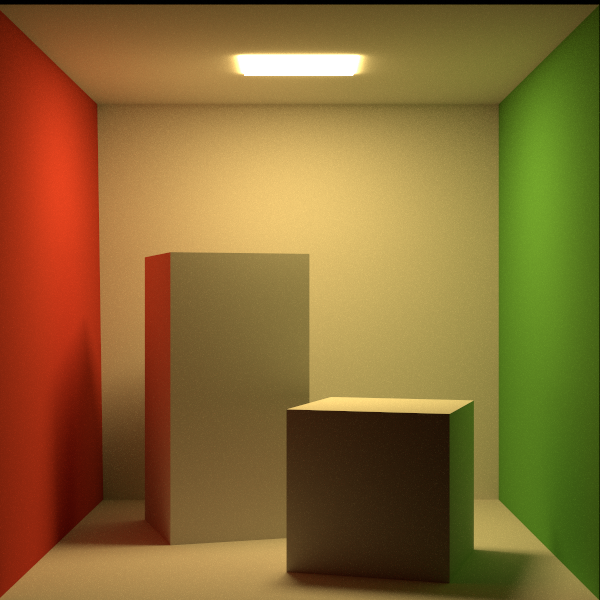
\includegraphics[width=\textwidth]{cornell_box_lux.png}
\end{subfigure}
\caption{Cornell Box rendered on our path tracer (\textit{left}), Blender Cycles 3.4.0 (\textit{middle}) and LuxCoreRender 2.61 (\textit{right}). All images were rendered at 600x600 resolution with a maximum of 4 diffuse bounces per sample.}
\label{img:cornell_box_comparison}
\end{figure}

With regards to performance, instead, the matter is significantly more complex; although we demonstrated that different renderers will eventually converge to the same image, how they get there and how long that takes is somewhat less predictable. A candidate metric to measure performance might be the average \textit{samples per second} value, but not all samples are created equal: a renderer may in fact be able to produce a cleaner image than a competitor's with fewer samples, by making use of superior importance sampling strategies. Ideally, we would measure noise at iso-time, or equivalently the time needed to reach a set noise level. While this feature might be available separately in the individual renderers (like with Cycles'  or LuxCoreRender's \textit{Noise Threshold} parameters), a cohesive and unique definition for "noise" is not easy to get by, and we ultimately renounced pursuing this method any further.

Luckily, the performance profile of our renderer and Cycles' came out to be very similar, and images produced at any given number of samples are almost equally noisy. This allowed us to revert to an easier metric to compare our path tracer's performance against commercial solutions, by timing the rendering process with a set sample count limit. The results of that comparison are reported in \Cref{img:render_times}, where our path tracer can be seen outperforming Cycles on the majority of the scenes we tested. The trend shows that the simpler the scene (like for the base Cornell Box which has just 32 triangles), the wider the performance margin in favor of our path tracer becomes, and conversely with more complex scenes (Sponza - 262269 triangles, Bmw - 699798 triangles) the render times get more similar between the two renderers.

\begin{figure}[h]
\centering
\includesvg[width=0.7\textwidth]{render_times.svg}
\caption{Results of the comparison of the absolute render times for the provided sample scenes between Blender Cycles 3.4.0 with CUDA backend (\textit{blue}) and our path tracer (\textit{red}), as rendered on a RTX 3060 at 800x600 with a target of 4096 samples (2048 for \texttt{sponza}).}
\label{img:render_times}
\end{figure}

The superior performance demonstrated by our path tracer compared to Cycles is most likely due to the latter renderer being infinitely more general and flexible: Cycles has support for any physically based material imaginable, and its BVH performance might be the result of a compromise between raw traversal speed and updatability, to more efficiently render animations where the geometry might not be static; this is a problem that our renderer just didn't consider. Cycles - like many other modern renderers - also supports an Optix backend in place of CUDA, which would be able to take advantage of ray tracing hardware acceleration built into many recent GPUs, and increase performance dramatically.

Finally, \Cref{img:nee_comparison} and \ref{img:bvh_perf} show the substantial quality and performance improvements brought by the algorithmic optimizations of Next Event Estimation and BVH respectively.

\begin{figure}[h]
\centering
\begin{subfigure}{0.45\textwidth}
\centering
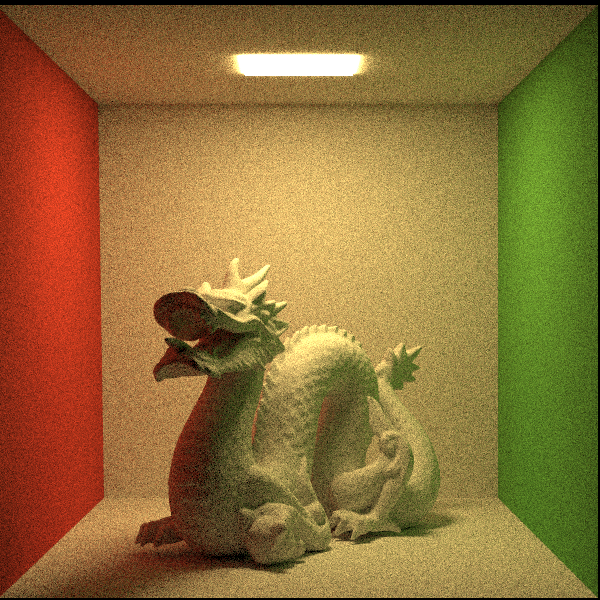
\includegraphics[width=\textwidth]{cornell_box_dragon_no_nee_1024.png}
\end{subfigure}
\hspace{0.4cm}
\begin{subfigure}{0.45\textwidth}
\centering
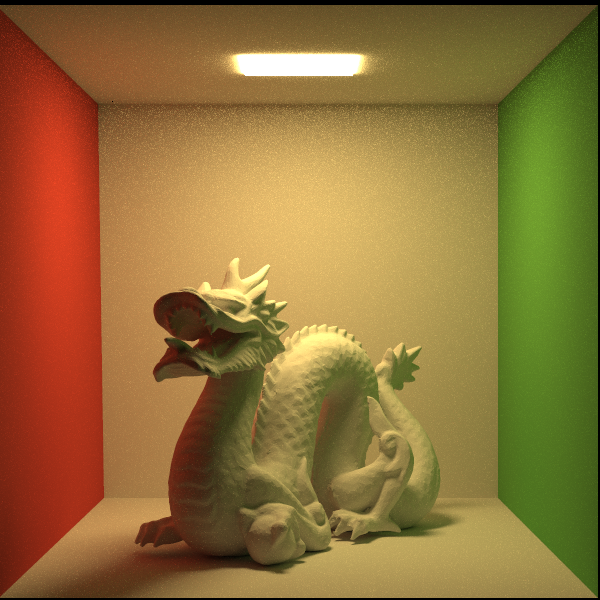
\includegraphics[width=\textwidth]{cornell_box_dragon_nee_1024.png}
\end{subfigure}
\caption{Difference between Next Event Estimation disabled (\textit{left}) and enabled (\textit{right}) on \texttt{cornell\_box\_dragon}, at 1024 samples for both images. As can be noted, the explicit light sampling version is significantly less noisy.}
\label{img:nee_comparison}
\end{figure}

\begin{figure}[h]
\centering
\includesvg[width=\textwidth]{bvh_perf.svg}
\caption{Comparison of relative performance with BVH enabled (\textit{blue}) and disabled (\textit{red}) for the provided sample scenes. As the triangle count increases, the sample rate quickly plummets without ray tracing acceleration structures.}
\label{img:bvh_perf}
\end{figure}

\section{Conclusions}

The project undoubtedly turned out to be quite successful, and the results have exceeded our best hopes. CUDA provided us with all the tools we could have needed, and its development environment was definitely more than adequate; tools such as Nsight Compute and its Visual Studio integrated debugger eased our jobs immensely, for example by allowing to set breakpoints in GPU code. The profiler also helped tremendously in measuring kernel execution times, and giving useful advice on how to mitigate inefficiencies, which helped us get close or beat the performance level of competing solutions.

Even though we showed how critical techniques such as next event estimation and an appropriate ray tracing acceleration structure can be, there would be a lot of work required to bring this proof of concept renderer to feature parity with commercial-grade products. In the first place, a path tracer approach to solving the rendering equation is hardly the best choice overall when alternatives such as Metropolis Light Transport exist, which could be able to solve "difficult" effects such as caustics while possibly having faster convergence times. Then, most of the work would be needed to model a wider range of materials, by adding support for more BRDFs and BSDFs (\textit{Bidirectional Scattering Distribution Function}, a more general form of the BRDF that also considers subsurface scattering); this is called \textit{Phisically Based Rendering} (\textit{PBR}) in the industry. The rest of the shortcomings are things like Multiple Importance Sampling (an extension of next event estimation which considers different criteria when choosing the next direction), vertex attribute interpolation (which could enable smooth shading and texture mapping), volumetric rendering, realistic camera properties such as bokeh effect, etc.

\printbibliography

\end{document}
